\subsection{Introduction and Background}
A key aspect of measuring distance with sound is the ability to reliably reproduce a high power and accurate audio tone. The tone produced should have a high SPL output such that it can be detected from far away, and should be accurate such that the tone can be extracted at the receiver in the midst of background noise. The designed system should also have an easy to use control system for testing a wide range of tones. This section of the report covers the development of the speaker system, looking at the speaker and amplifier, the creation of a sine wave and code development for controlling the system.\\
\subsection{Hardware}
\subsubsection{Microcontroller}
The chosen MCU for testing the system is the Teensy 4.0. This was chosen as it has clock rates of up to 600MHz which can be reduced down to match the clock rate of the MCU used in the final product.
\subsubsection{Speaker}
The used speaker for the system is the AS01508MS-SP11-WP-R as it was supplied by the sponsor. This has the specifications shown in Table \ref{tab:L_speakerSpecs}.  The system designed for the speaker needed to supply at least 0.7W, and to get the highest SPL from the speaker it needs a supply of at least 1W. \\

Other characteristics of importance for the speaker include the impedance and sensitivity, which are both functions of frequency. Each component selected in the design for the speaker system took into account this frequency response, selecting components with a similar frequency response. \\

\begin{table} [!htb]
	\caption{Key speaker specifications, source: \cite{speakerDatasheet}}
	\label{tab:L_speakerSpecs}
	\centering
	\begin{tabular}{ |c|c|c| }
		\hline
		Parameter & Value & Unit \\ 
		\hline
		Rated Input Power & 0.7 & W \\ 
		Max Input Power & 1 & W \\ 
		Impedance & 8 $\pm$ 15\% & Ohms \\
		Sensitivity (SPL@2V/10cm) & 89 $\pm$ 3 & dB \\
		\hline
	\end{tabular}
\end{table}

\subsubsection{Amplifier}
The output from the MCU is a 3.3V peak waveform with a 0.04mA current, this is a much lower power output than what is needed by the speaker. An amplifier is used to increase the power of the output waveforms from the MCU. \\

There were several options considered for the amplifier, class A, class B, class AB and class D each with their own advantages and disadvantages. Ultimately, the best amplifier for the system is the class D amplifier. This is because it is more efficient than the other options (theoretically up to 100\%), allowing the speaker to be driven to its peaks. Efficiency is also important to meet the low power draw user requirement of the system. \\

The chosen amplifier is the class D PAM8403 audio amplifier with the specifications shown in Table \ref{tab:L_ampSpecs}. The amplifier was chosen as it is up to 90\% efficient outputting up to 1.4W for the 8$\Omega$ load. The amplifier gets its efficiency using differential outputs and sinusoidal PWM to pull each leg of the speaker between 0 and 5V.\\
\begin{table} [!htb]
	\caption{Key amplifier specifications, source: \cite{amplifierDatasheet}}
	\label{tab:L_ampSpecs}
	\centering
	\begin{tabular}{ |c|c|c| } 
		\hline
		Parameter & Rating & Unit \\ 
		\hline
		Input Voltage & -0.3 to +0.3 & V \\ 
		Supply Voltage & 5.0 & V \\ 
		Output Power for 8 $\Omega$ Load and 5V Supply & 1.4 & W \\
		\hline
	\end{tabular}
\end{table}

Getting high a high output waveform from the amplifier is key for producing a loud tone. The 1.4W output is too high for the speaker though, so it is reduced on the input to the amplifier. This is done using a 10k variable resistor which essentially acts as a volume knob. Putting this at the entrance of the amplifier also protects the amplifier, as the amplifier is rated for -0.3V to 0.3V input but the MCU outputs 3.3V peak. Reducing the waveform here also reduces the power loss as the current is small. The schematic for the amplifier circuit is shown in Figure \ref{fig:L_amplifier}.
\begin{figure} [!htb]
	\captionsetup{justification=centering}
	\hfill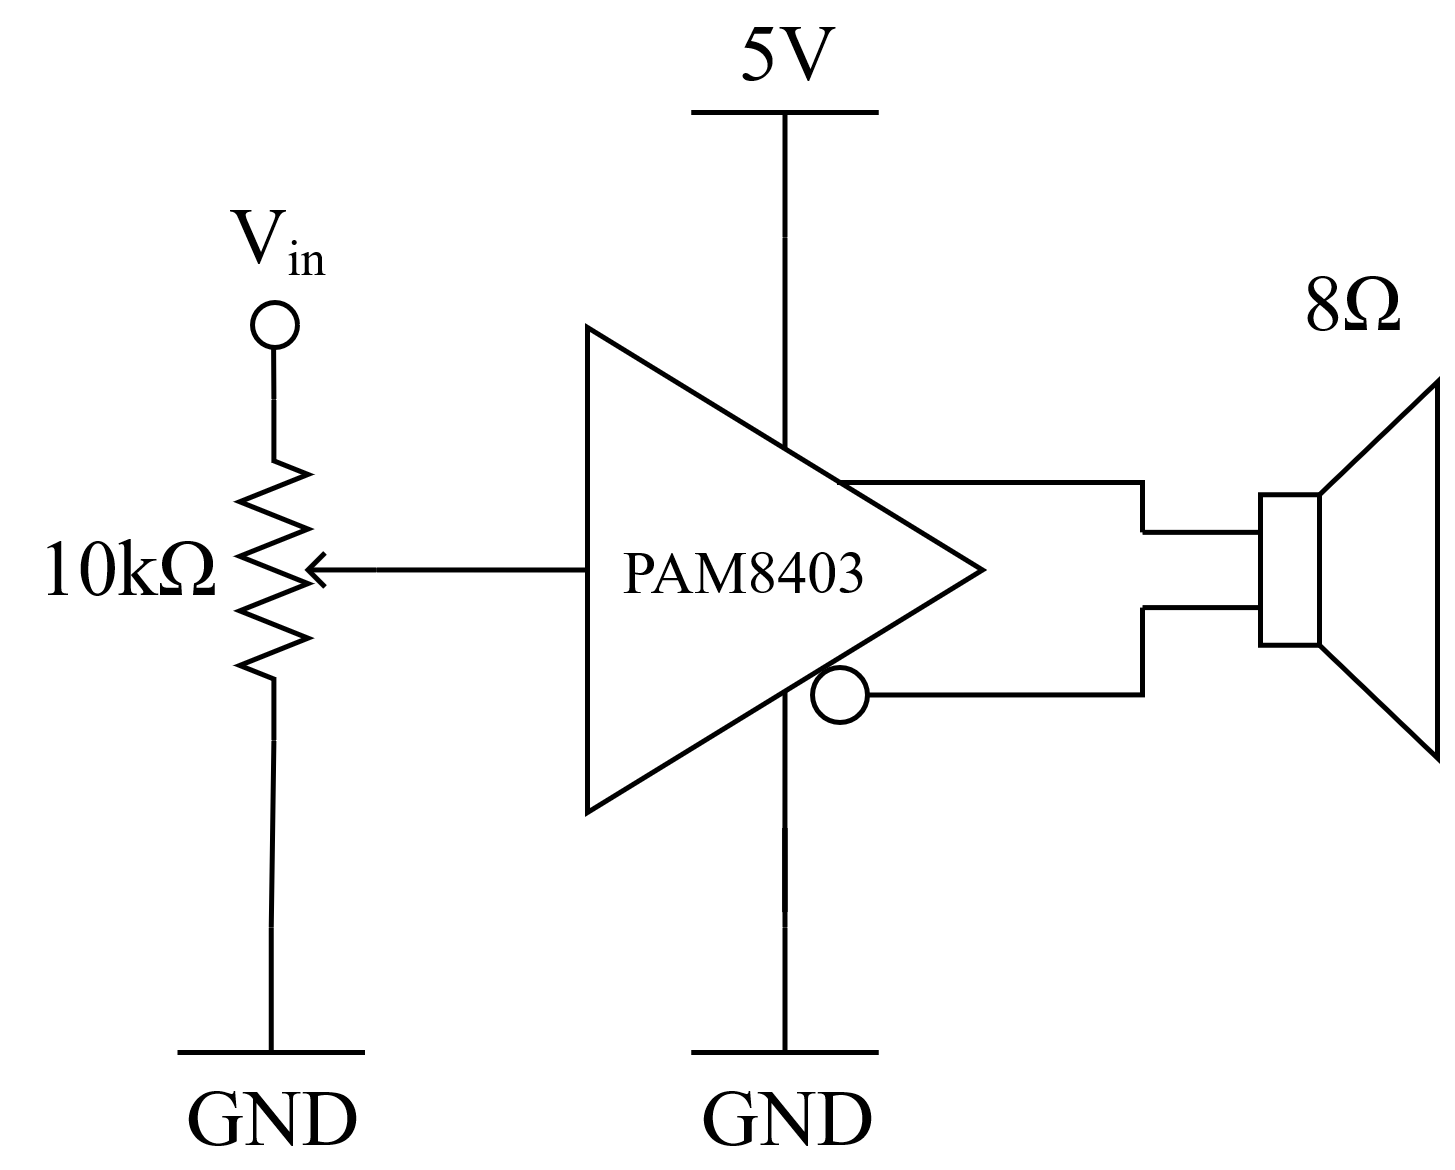
\includegraphics[width=0.4\textwidth]{./images/speaker/L_Amplifier}\hspace{\fill}
	\caption{Speaker and audio amplifier schematic with 10k$\Omega$ volume knob}
	\label{fig:L_amplifier}
\end{figure}

\subsection{Playing Tones}
A square tone can easily be played by running a 50\% duty cycle PWM waveform through the speaker. The problem with square tones, however, is that they contain an infinite number of harmonics. If a square waveform is passed through the speaker, then it is hard to determine exactly what the output waveshape will be. For trying to produce an accurate output waveform, the system needs to be able to play sinusoidal waveforms. \\

The Teensy 4.0 MCU chosen for the project cannot easily produce a sinusoidal tone as it does not include a digital to analogue converter. To get around this there were several options considered including purchasing an off-board DAC, purchasing a new MCU, or using code to produce sinusoidal PWM. The best option was to use parts that were easily obtained to meet the low-cost user requirement, that meant using sinusoidal PWM. By generating a sinusoidal PWM signal, and passing the waveform through a low pass filter, a good estimate of a sine wave can be produced. \\
\subsubsection{Generating Sinusoidal PWM}
\label{sec:L_Sinusoidal PWM}
First the sinusoidal PWM waveform needs to be generated at the MCU output pin. This was done using code. A continuous sinusoidal waveform of period, $T_s$, is split up into $L$ discrete intervals. At each of these intervals, the duty cycle increased or decreased by $\frac{100\%}{2^m}$ where m is the resolution of the PWM generator. 100\% duty cycle is equal to $2^m - 1$, which is set when the sinusoid is at its peak, and the minimum value corresponding to 0\% duty cycle is 0 which is set when the sinusoid is at its minimum. The 50\% duty cycle is then $(2^m-1)/2$ which is the cross-over point of the sinusoid. These values are put into a sine look up table of length L. Figure \ref{fig:L_Sinusoidal_PWM} shows this method. \\

\begin{figure} [!htb]
	\hfill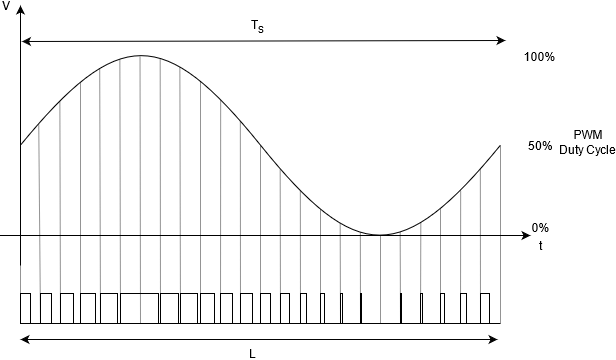
\includegraphics[width=0.45\textwidth]{./images/speaker/L_Sinusoidal_PWM}\hspace{\fill}
	\caption{Sinusoidal PWM generation}
	\label{fig:L_Sinusoidal_PWM}
\end{figure}
To set the rate which the LUT is indexed, a counter and an interrupt timer is used. At each interrupt period, $\tau$, a step of $\Delta$ is added to the current counter value. Once the counter exceeds the maximum counter value, $M$, the counter is reset with remainder carried and the LUT is indexed by one for each amount of $\Delta$ the count is above M. Figure \ref{fig:L_Counter} shows the visualisation of the counter. 
\begin{figure} [!htb]
	\captionsetup{justification=centering}
	\hfill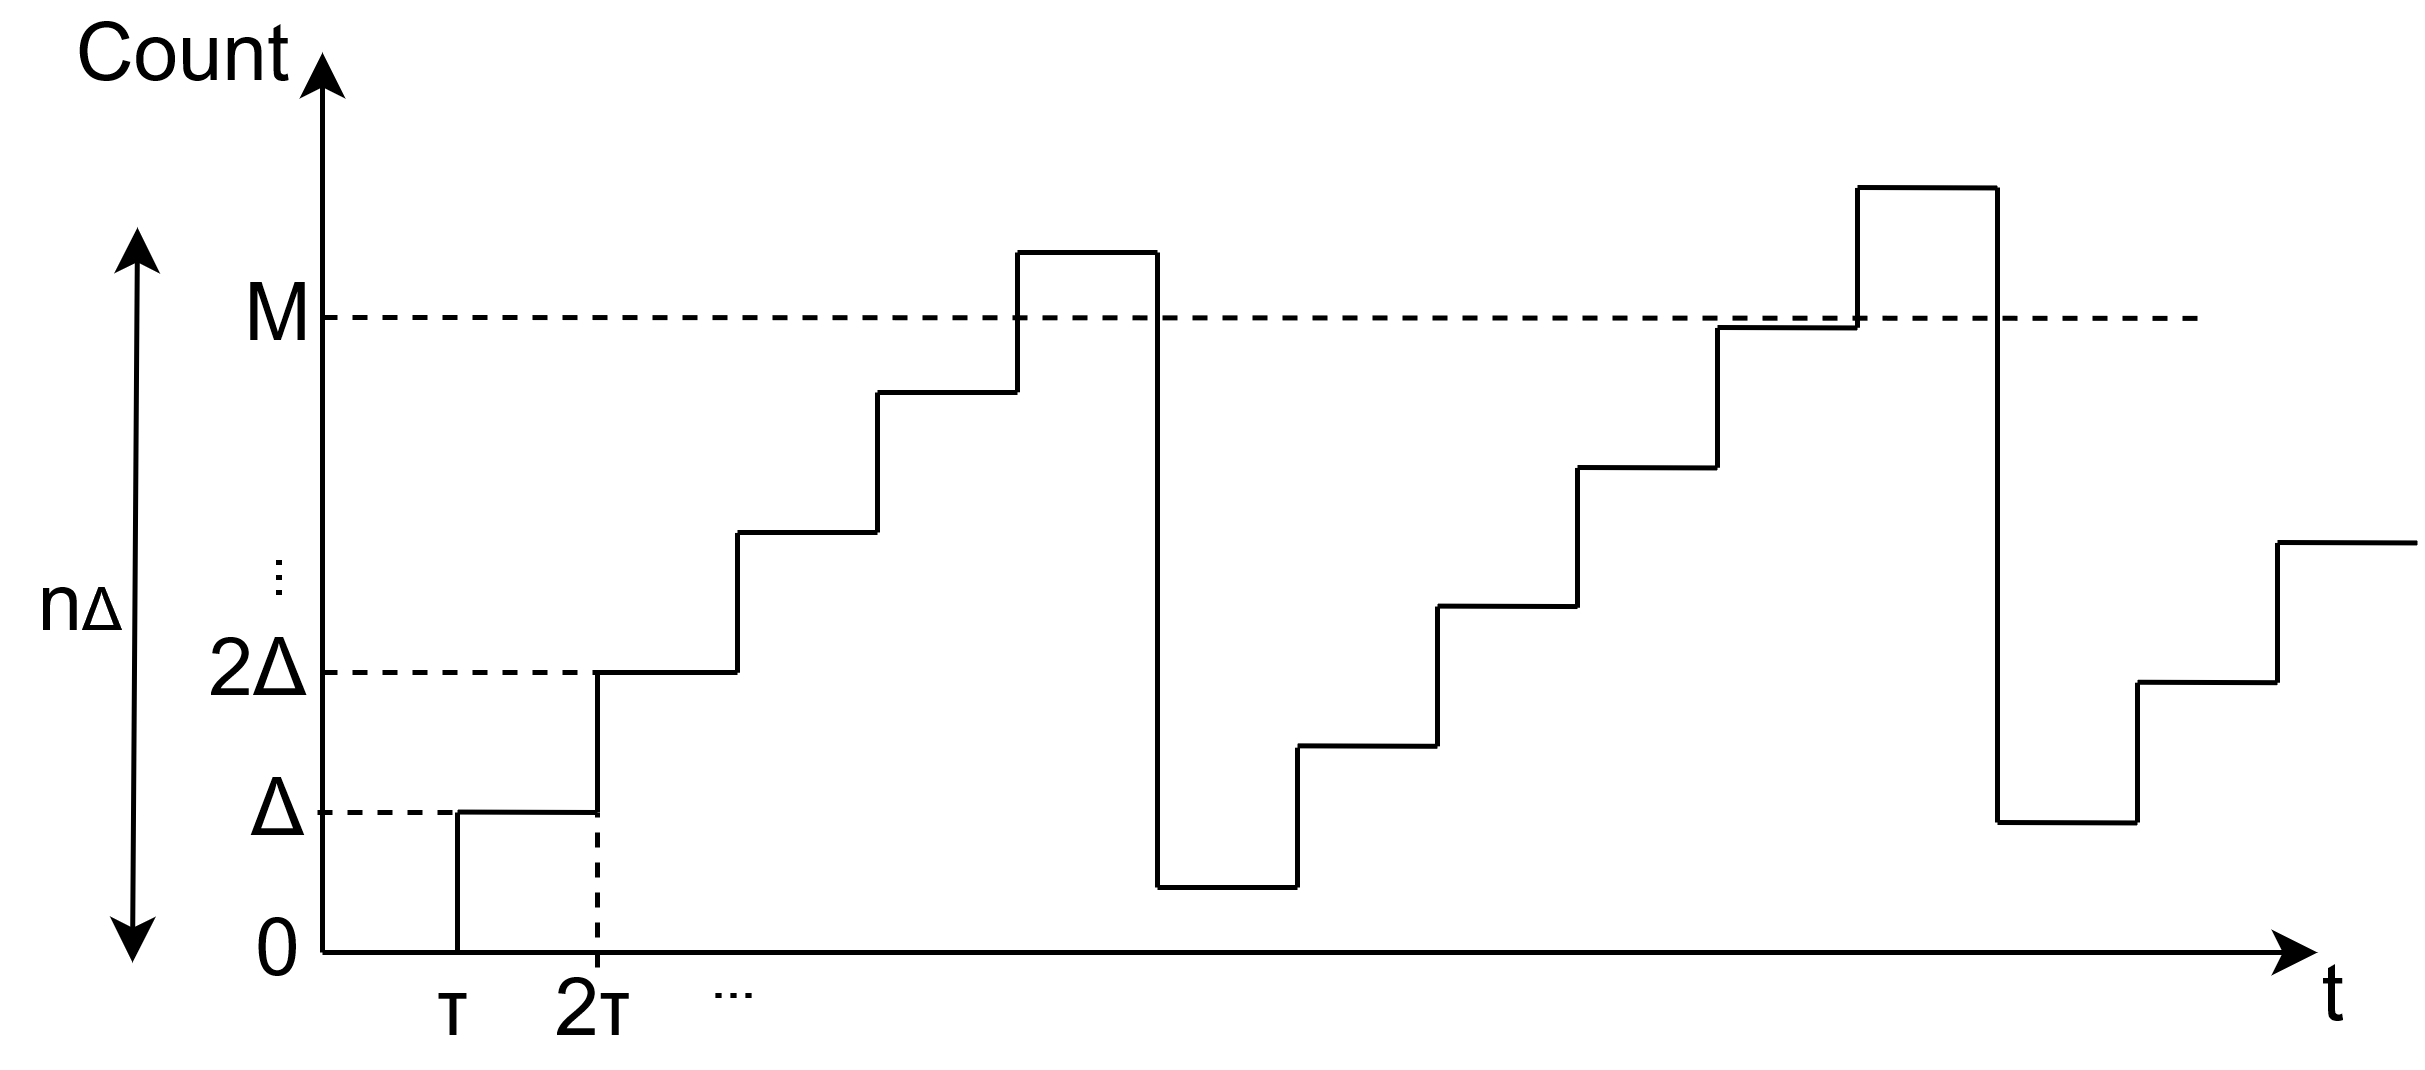
\includegraphics[width=0.45\textwidth]{./images/speaker/L_Counter}\hspace{\fill}
	\caption{Counter with max value M, it takes n$\Delta$ counts to exceed M}
	\label{fig:L_Counter}
\end{figure}

It takes $n$ lots of $\Delta$ to exceed $M$ therefore:
\begin{equation}
	n\times\Delta \ge M \implies n = \frac{M}{\Delta}
	\label{eqn:M/D}
\end{equation}
The interrupt is being called every $\tau$ seconds and so the time it takes per increment of the LUT is $n\times T$. There are $L$ elements in the LUT so, the period of the sine wave is thus:
\begin{equation}
	T_s = n\times \tau\times L
\end{equation}
Which can be written in terms of frequency:
\begin{equation}
	f_s = \frac{1}{n\tau L}
\end{equation}
And in terms of the step size by substituting equation \ref{eqn:M/D}:
\begin{equation}
	f_s(\Delta) = \frac{\Delta}{M\tau L}
\end{equation}

The frequency of the output sine is now a function of the step size $\Delta$ and thus sinusoidal waveforms of selectable frequencies can be produced. The equation can be re-arranged to find any values of $\Delta$ that gives a corresponding sinusoidal output frequency, which is how the code decides the output frequency. \\

The values of M and $\tau$ were determined through experimentation where if the interrupt rate is higher than the  interrupt handler function then frequency gets capped at less than 20kHz. Having the interrupt rate too low would result in the same problem. The value for $f_{PWM}$ was chosen as such as it allows the PWM frequency to be fully filtered out leaving behind just the sinusoidal component. The value of m is dependent on the PWM frequency and vice-versa, however the Teensy can re-map values passed to it, so the selection of m is irrelevant and a value of 8 is used. Finally, the LUT was selected as $2^8$ to match the PWM resolution used. The values selected for the sinusoidal PWM generation parameters are summarised in Table \ref{tab:L_sinusoidalPWM}.\\
\begin{table} [!htb]
	\caption{Parameters used for sinusoidal PWM generation}
	\label{tab:L_sinusoidalPWM}
	\centering
	\begin{tabular}{ |c|c|c|c| }
		\hline
		Parameter & Description & Value & Units \\ 
		\hline
		M & Counter Maximum & 100 & - \\ 
		$\tau$ & Interrupt Period & 5 & $\mu$s \\ 
		L & LUT Size & $2^8$ & - \\
		$f_{PWM}$ & PWM Frequency & $2^8\times f_s$ & Hz\\
		m & PWM Resolution & 8 & - \\
		\hline
	\end{tabular}
\end{table}

\subsubsection{Filtering the Sinusoidal PWM Signal}
\label{sec:L_Low_Pass_Filter}
To filter the sinusoidal PWM signal, a second order LC Butterworth filter is used. The filter connects to the output pin on the MCU as shown in Figure \ref{fig:L_LPF}. The values selected for the LPF gives the filter a cut-off frequency of 28kHz. 28kHz was chosen as it higher than the maximum frequency of the speaker but is also able to fully filter out the PWM carrier frequency. \\

The filter also contains a 67$\mu$F electrolytic capacitor. This is because the output sinusoidal PWM waveform generated is shifted with a maximum value of 3.3V and a minimum value of 0V. To get the speaker driven to the peaks in its motion it needs to be fed a waveform centred about DC. So using a DC blocking capacitor shifts the output sine waveform from the LPF back to DC. The capacitor and the 10k$\Omega$ resistor at the entrance of the amplifier form a passive bandpass filter with a passband of between 0.237Hz and 297Hz depending on the position of the variable resistor wiper, and a stopband of 28kHz. \\
\begin{figure} [!htb]
	\hfill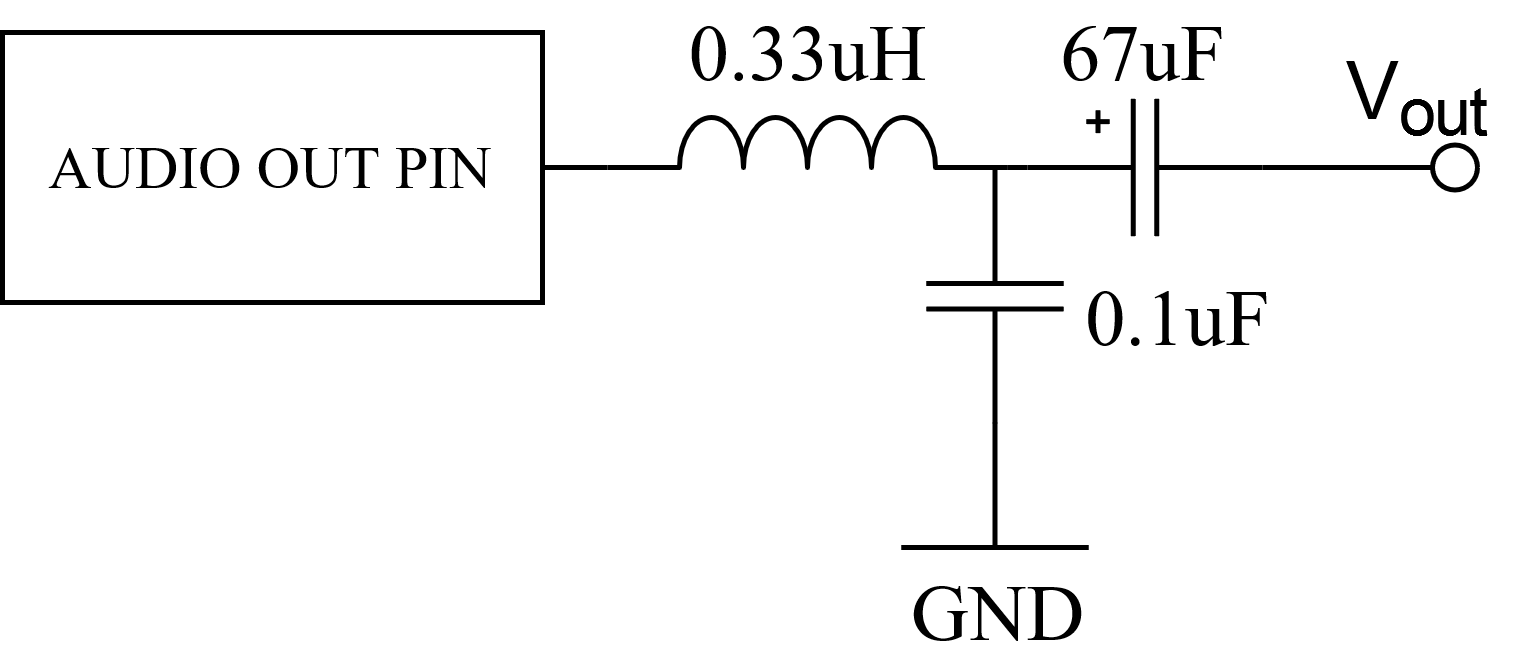
\includegraphics[width=0.5\textwidth]{./images/speaker/L_LPF}\hspace{\fill}
	\caption{Second order LC low pass filter with a cut-off frequency of 28kHz}
	\label{fig:L_LPF}
\end{figure} 

\subsubsection{Linear FM Sweep (Chirp)}
\label{sec:L_Chirps}
The speaker is required to play a linear FM sweep as used in the convolution method of measuring distance. To produce a linear FM sweep, or chirp, the continuous function is described by:
\begin{equation}
	f(t) = ct + f_0
	\label{eqn:Chirp1}
\end{equation}
Where $f_0$ is the initial frequency, and c is the chirp rate, calculated as:
\begin{equation}
	c = \frac{f_1 - f_0}{T_c}
\end{equation}
Where $f_1$ is the final frequency and $T_c$ is the sweep or chirp time. \\

The sinusoidal PWM frequency output is a function of the step size, $\Delta$, and interrupt period $\tau$ as outlined in section \ref{sec:L_Sinusoidal PWM}. To do a linear FM sweep like that in equation \ref{eqn:Chirp1}, the time step is first discretised. This is done by dividing the chirp time, $T_c$, by the interrupt period, $\tau$, finding the number of interrupt calls within the chirp duration: \\
\begin{equation}
	n = \frac{T_c}{\tau}
\end{equation}
At each interrupt call, the frequency of the sinusoidal PWM waveform is increased by adding a "step-step" value to the current value of the step size. The step-step value is calculated as:
\begin{equation}
	\Delta_\Delta = \frac{\Delta_1 - \Delta_0}{n} 
\end{equation}
Where:
\begin{equation*}
	\Delta_0 = f_0ML\tau; \Delta_1 = f_1ML\tau
\end{equation*}
Now given any two frequencies, a sinusoidal PWM linear FM sweep can be generated. Each frequency is played for a nth of the total chirp. Filtering the output will produce a sinusoidal linear FM sweep. \\



\subsection{Code Development and System Control}
\subsubsection{Main Code}
The hardware is setup in such a way that there is a huge amount of freedom in what the speaker can play. To play the right tone for testing, a system was designed for the code that essentially allows users to "program" from within the serial interface. The code reads from the serial interface and compares the input to a pre-defined list of functions. The code then extracts the inputs from the function and processes the inputs. If there is any errors with the serial input then the code will simply spit out an error, preventing the MCU from locking. Figure \ref{fig:L_Code_Loop} shows the flowchart for this segment of code. The code was all written in C++ and was provided to the sponsor in section "Speaker/Speaker Programming/Speaker\_Code\_V4". \\
\begin{figure} [!htb]
	\hfill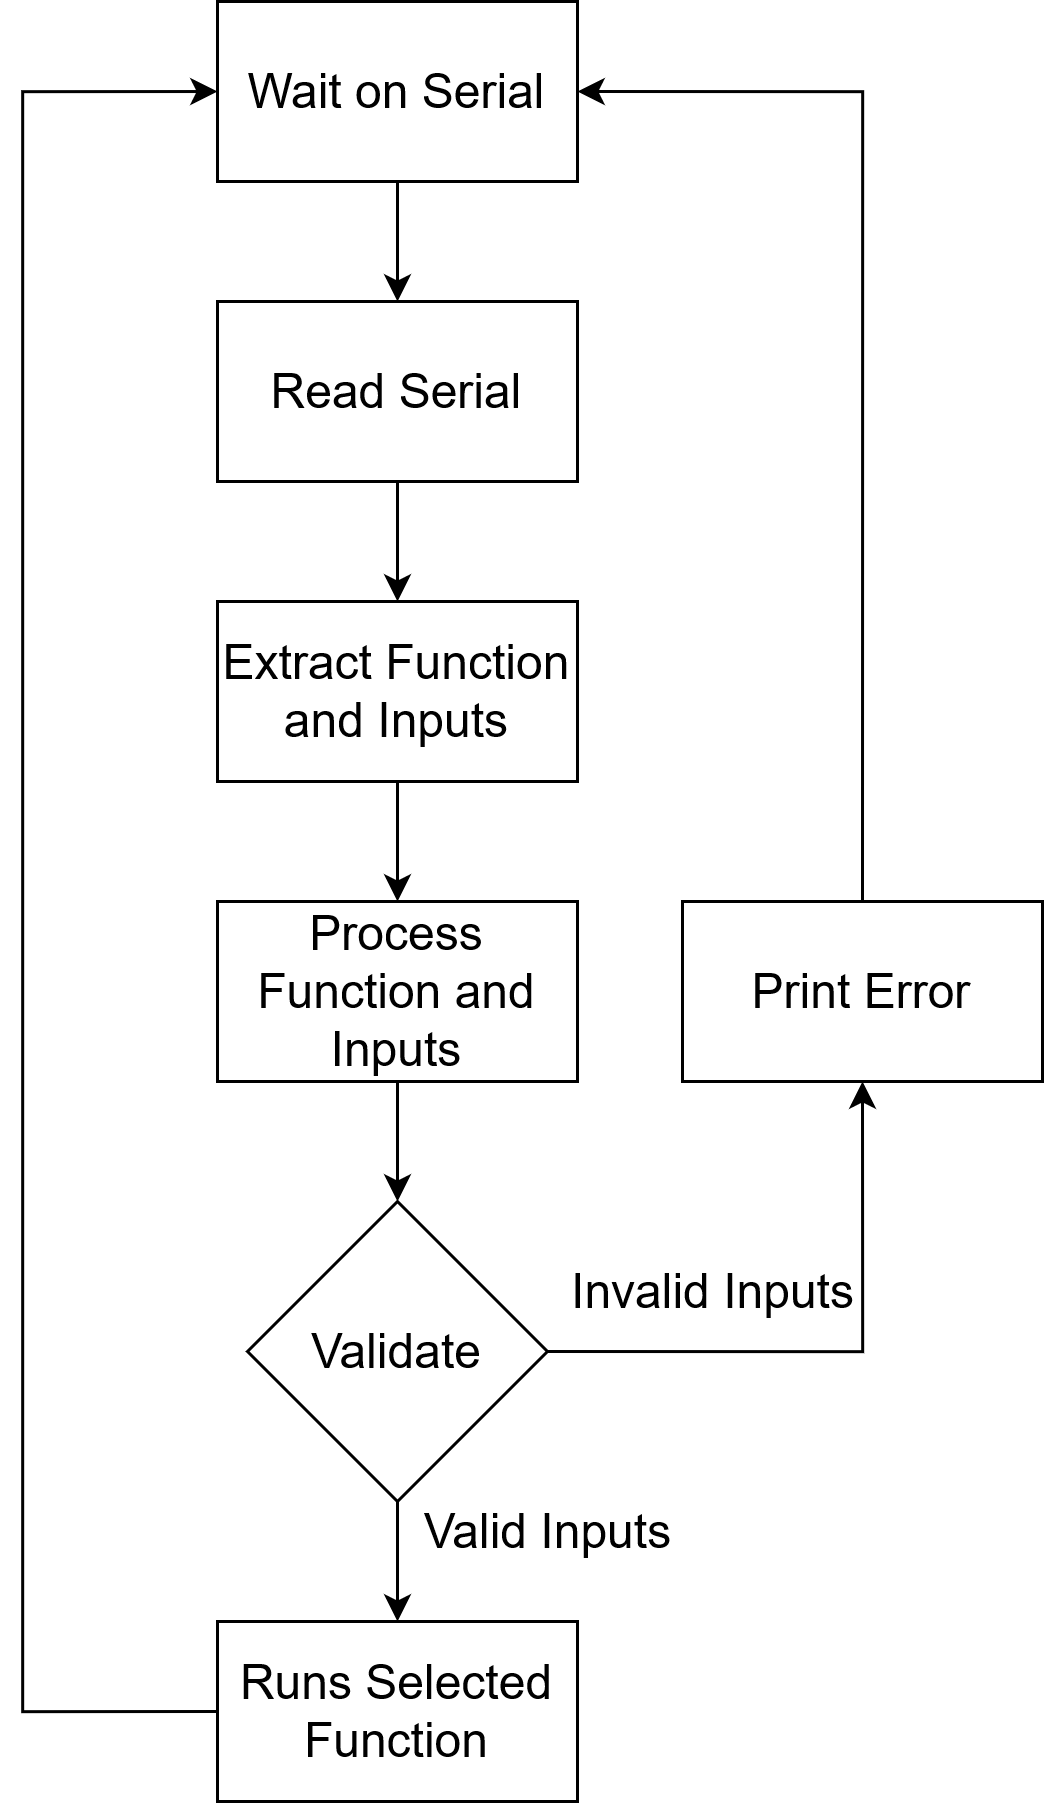
\includegraphics[width=0.4\textwidth]{./images/speaker/L_Code_Loop}\hspace{\fill}
	\caption{Code loop for reading from serial}
	\label{fig:L_Code_Loop}
\end{figure} 

To differentiate serial inputs, the function needs to be input between $<$ and $>$. The code waits until it detects the $<$ and will extract all the data from between the two arrows. Using this method allows the user to run several inputs at once in one serial line. When it comes to playing a tone, this allows the ability to run multiple one after the other essentially chaining waveforms together. \\

\subsubsection{Waveforms}
The code loop is combined with "waveforms", where each waveform is a struct stored in a singly linked list. Each waveform contains an an initial frequency, a final frequency, a wave time and a shape (p for square or s for sine). When the waveform is created it is given a unique identifier and is stored at the head of a singly linked list shown in Figure \ref{fig:L_Waveforms}. Waveforms in the list can be displayed, edited, deleted, played or even looped using functions outlined in Table \ref{tab:L_transmitterInteractions} in Appendix \ref{sec:l_append}. \\

\begin{figure} [!htb]
	\hfill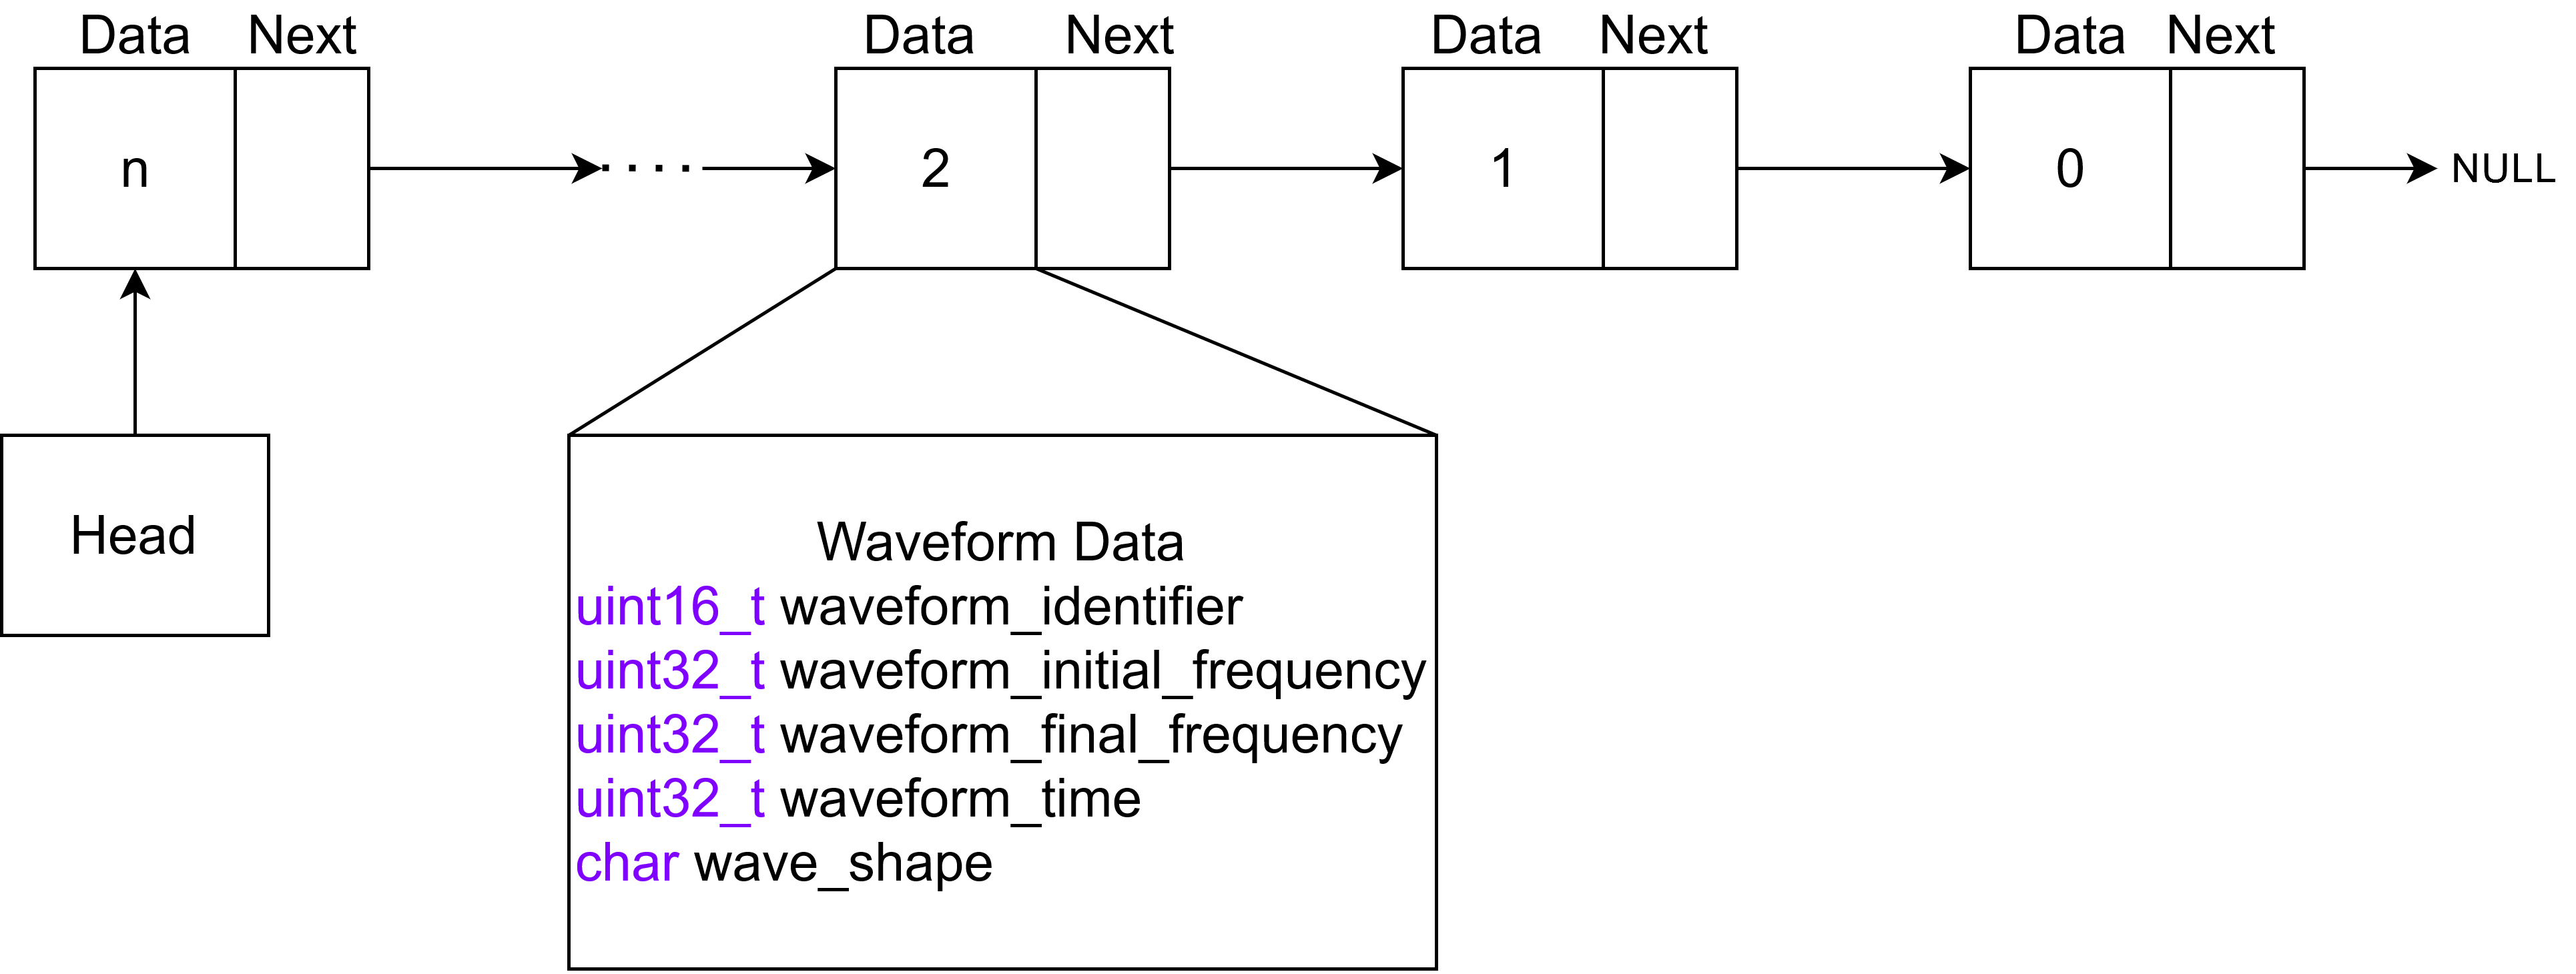
\includegraphics[width=\textwidth]{./images/speaker/L_Waveforms}\hspace{\fill}
	\caption{Waveforms in a linked list data structure}
	\label{fig:L_Waveforms}
\end{figure} 

Waveforms allow a convenient method of playing a wide range of tones quickly. For example, the user can create 10 waveforms of increasing frequency and test each one. After testing each one they could identify the best for the use case and keep on testing that one, typing in an identifier instead of each waveform property each time. For quick testing however, functions were created which allows users to simply input all the waveform properties without having to create a waveform. The play tone functions are outlined in Table \ref{tab:L_toneInteractions} in Appendix \ref{sec:l_append}. \\

\subsubsection{Transmitter}
The speaker system and code is integratead the main system by acting as the "transmitter". The transmitter is an object with a waveform, a delay period and an output pin. When told to transmit, the transmitter pulls a line high, transmits the waveform, waits a delay period, and then pulls the line low again. Pulling the line high allows the receiver to detect that the transmitter is about to transmit and can thus record the time and start running some receiver code. The transmitter also has some serial functions that are useful in testing, outlined in Table \ref{tab:L_transmitterInteractions} in Appendix \ref{sec:l_append}.
\pagebreak
\subsection{Results}
The hardware is split up into four components: the Teensy MCU development board, the bandpass filter board, the audio amplifier and the speaker itself. The hardware is connected as shown in Figure \ref{fig:L_Hardware} where the purple wire is the audio signal connecting to the audio output pin (3 in this case, can be set in code), the red wire is the amplifier power which connects to the 5V output of the Teensy and the black wire is ground which plugs into the ground connection on the Teensy. \\

\begin{figure} [!htb]
	\captionsetup{justification=centering}
	\hfill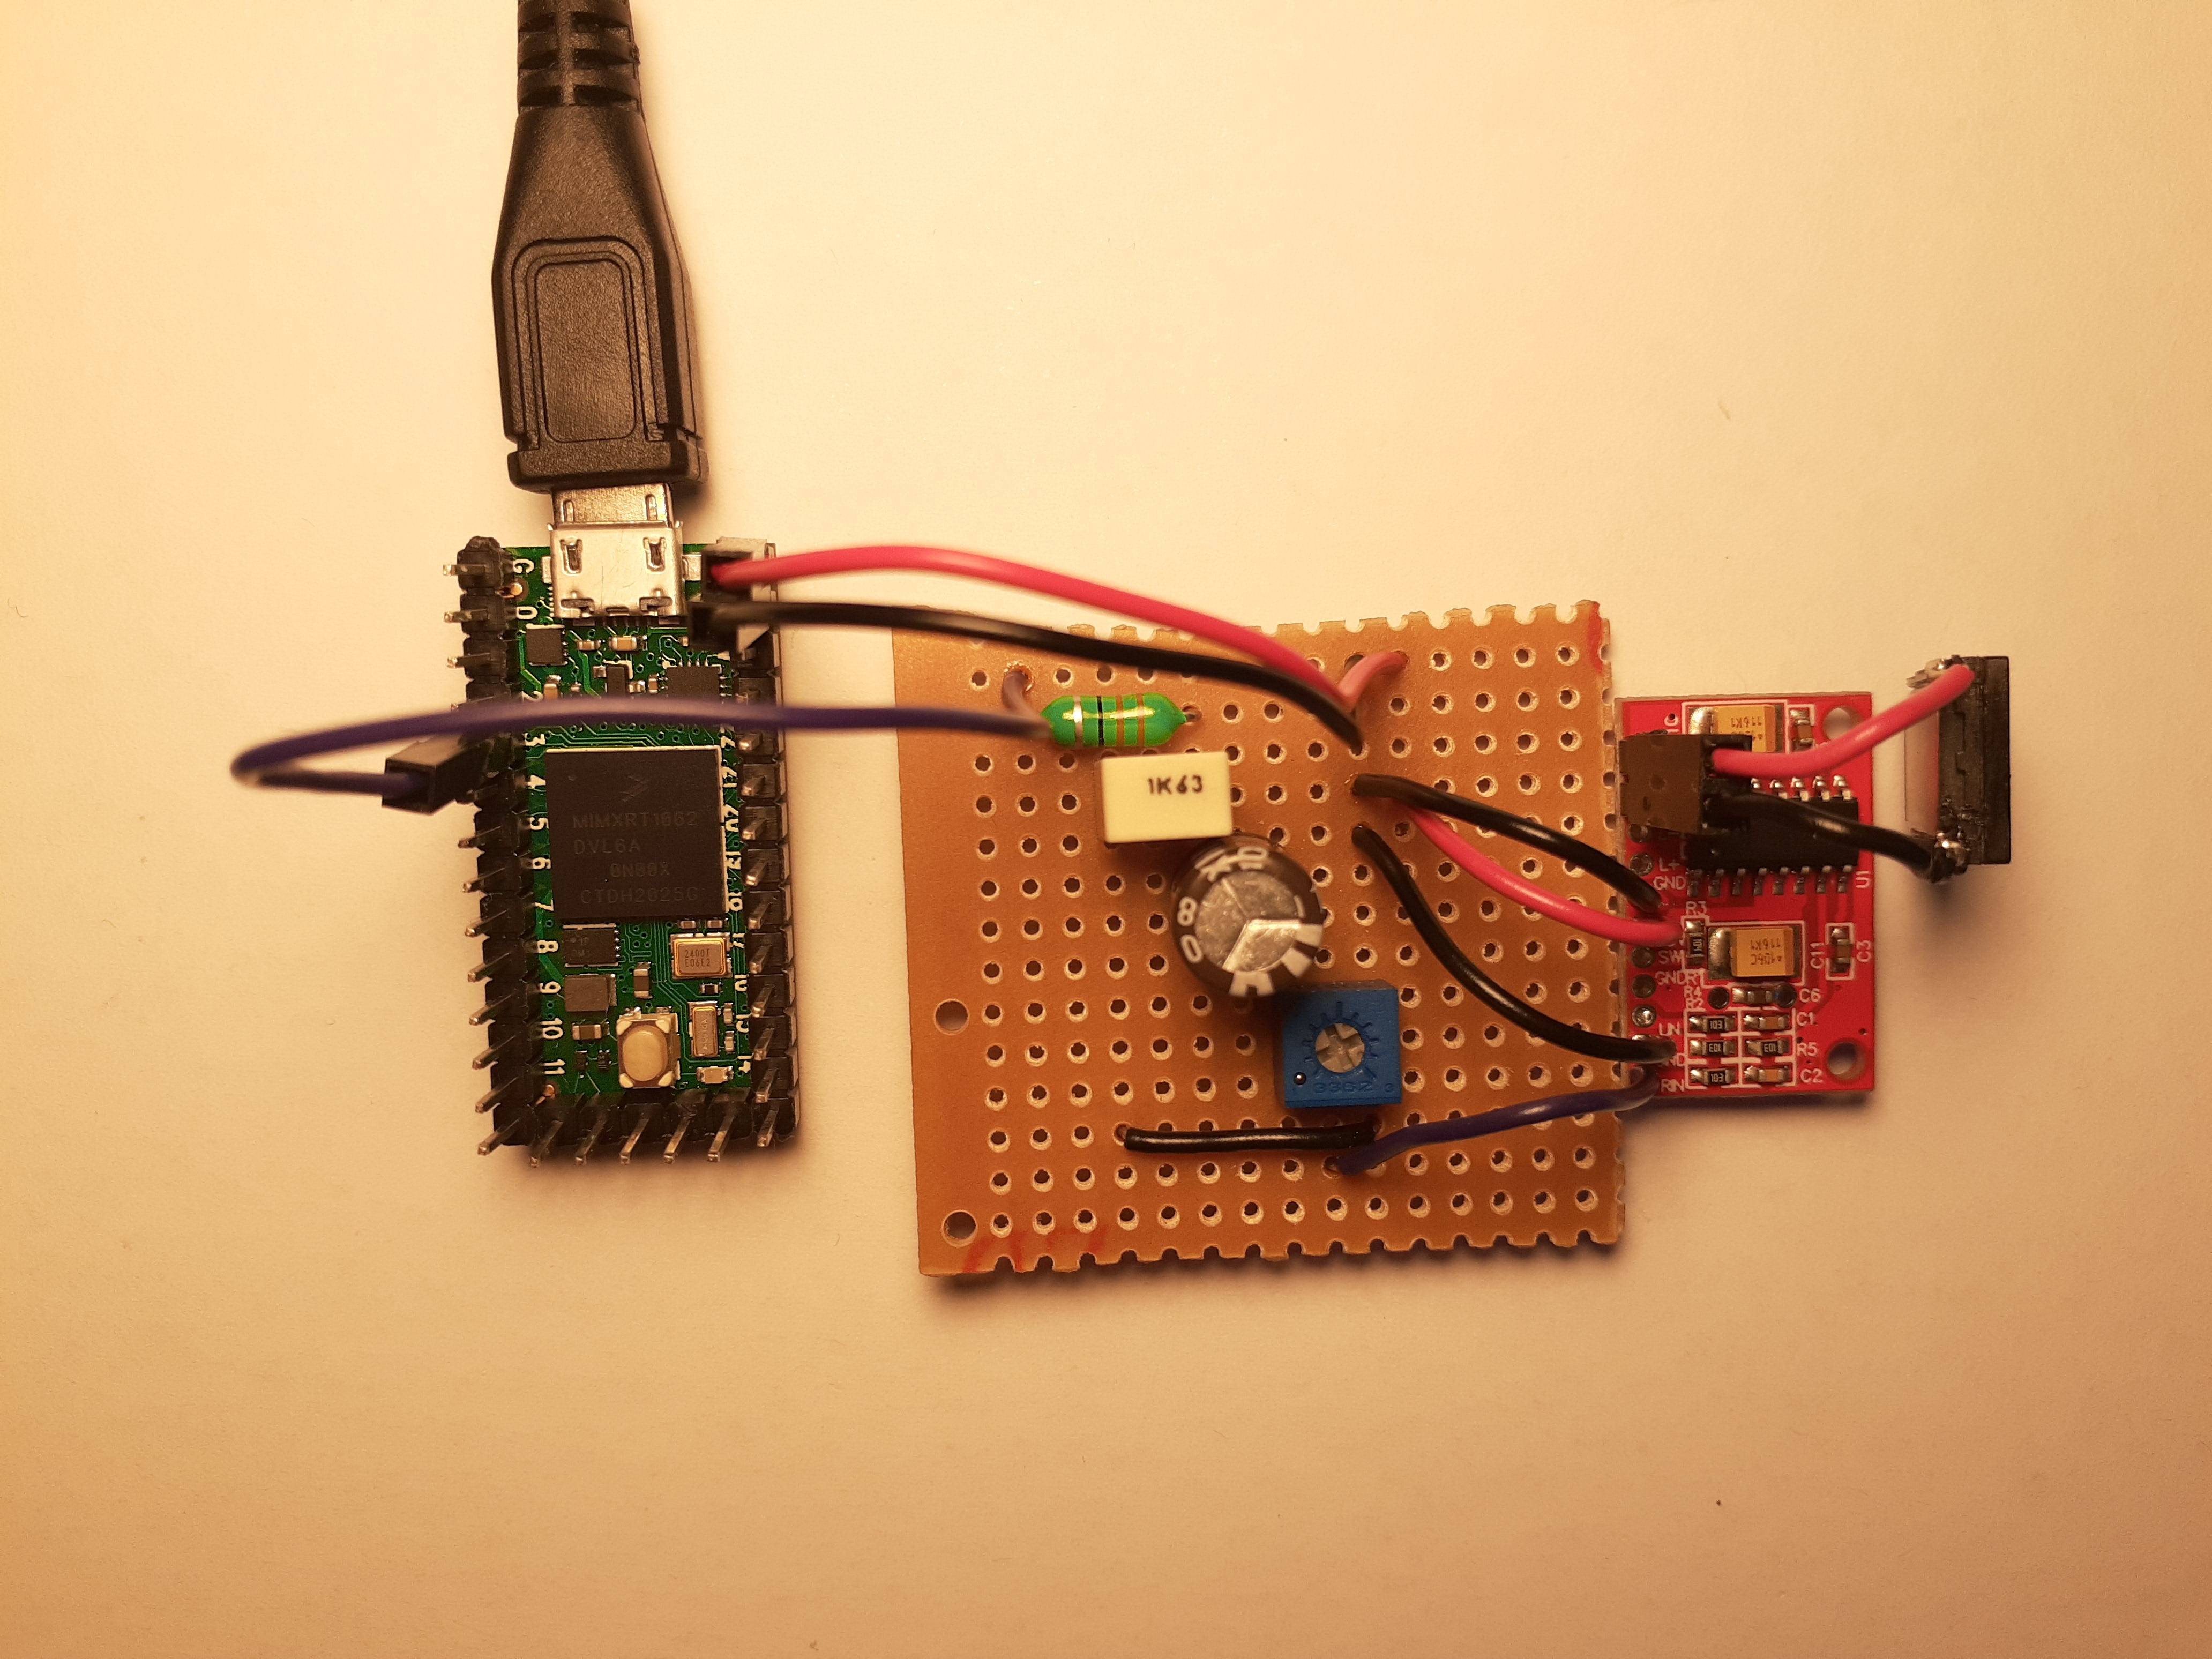
\includegraphics[width=0.4\textwidth]{./images/speaker/L_Hardware}\hspace{\fill}
	\caption{Speaker hardware setup, the labelled sections are - A: Teensy 4.0 MCU dev board, B: LPF and variable resistor volume knob, C: class D audio amplifier breakout board, D: Speaker}
	\label{fig:L_Hardware}
\end{figure} 

A wide range of tones were tested with the speaker, both square and sinusoidal. The system was capable of playing square tones up to 9kHz but not above as the extra harmonics were fully filtered. As the best range of the speaker is at 10kHz, this was the most tested waveform. The following results section shows the generation of a 10kHz tone from transmitter to receiver. \\

The waveform is first created and played shown in Figure \ref{fig:L_Create_Waveform}. The 1280 number shown is the step size required to play the 10kHz tone. The sinusoidal PWM waveform is then generated at the audio output pin shown in Figure \ref{fig:L_Create_Waveform}. The waveform has a lot of ripple as the PWM frequency is so high (2.54MHz). \\

The waveform is then passed through the LPF and DC blocking capacitor resulting in the waveforms shown in Figure \ref{fig:L_Shifted_Waveform}. \\

The waveform then travels through the medium. Figure \ref{fig:L_Output} shows the spectrum of the output audio waveform generated in MATLAB and the power spectral density of the output waveform generated using an auto regressive Yule-Walker method. The audio clip was recorded in the students bedroom on a quiet afternoon, as such there is little noise. \\

\begin{figure} [!htb]
	\captionsetup{justification=centering}
	\hfill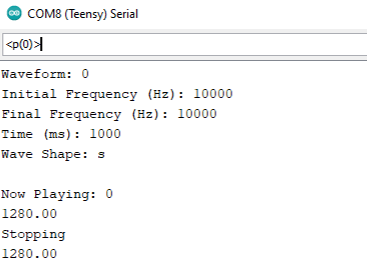
\includegraphics[width=0.45\textwidth]{./images/speaker/L_Create_Waveform}\hspace{\fill}
	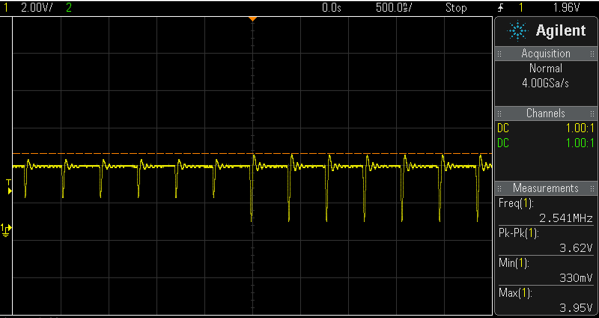
\includegraphics[width=0.5\textwidth]{./images/speaker/L_Generated_Sinusoidal_PWM}\hspace{\fill}
	\caption{Left: A 10kHz tone is created and given the unique identifer "0". The waveform is then played using the play function: $"<p(0)>"$. Right: The waveform as generated at the audio output pin.}
	\label{fig:L_Create_Waveform}
\end{figure}

\begin{figure} [!htb]
	\captionsetup{justification=centering}
	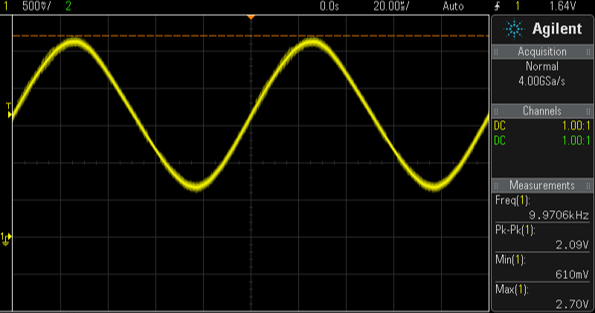
\includegraphics[width=0.5\textwidth]{./images/speaker/L_LPF_Output}
	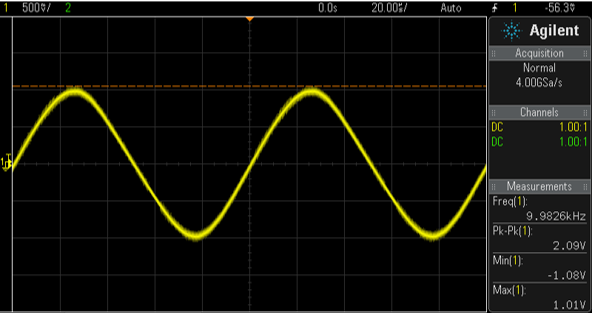
\includegraphics[width=0.5\textwidth]{./images/speaker/L_Shifted_Waveform}
	\caption{Left: the shifted waveform as seen at the exit of the LPF. Right: the waveform as seen at the exit of the DC blocking capacitor}
	\label{fig:L_Shifted_Waveform}
\end{figure}

\begin{figure} [!htb]
	\captionsetup{justification=centering}
	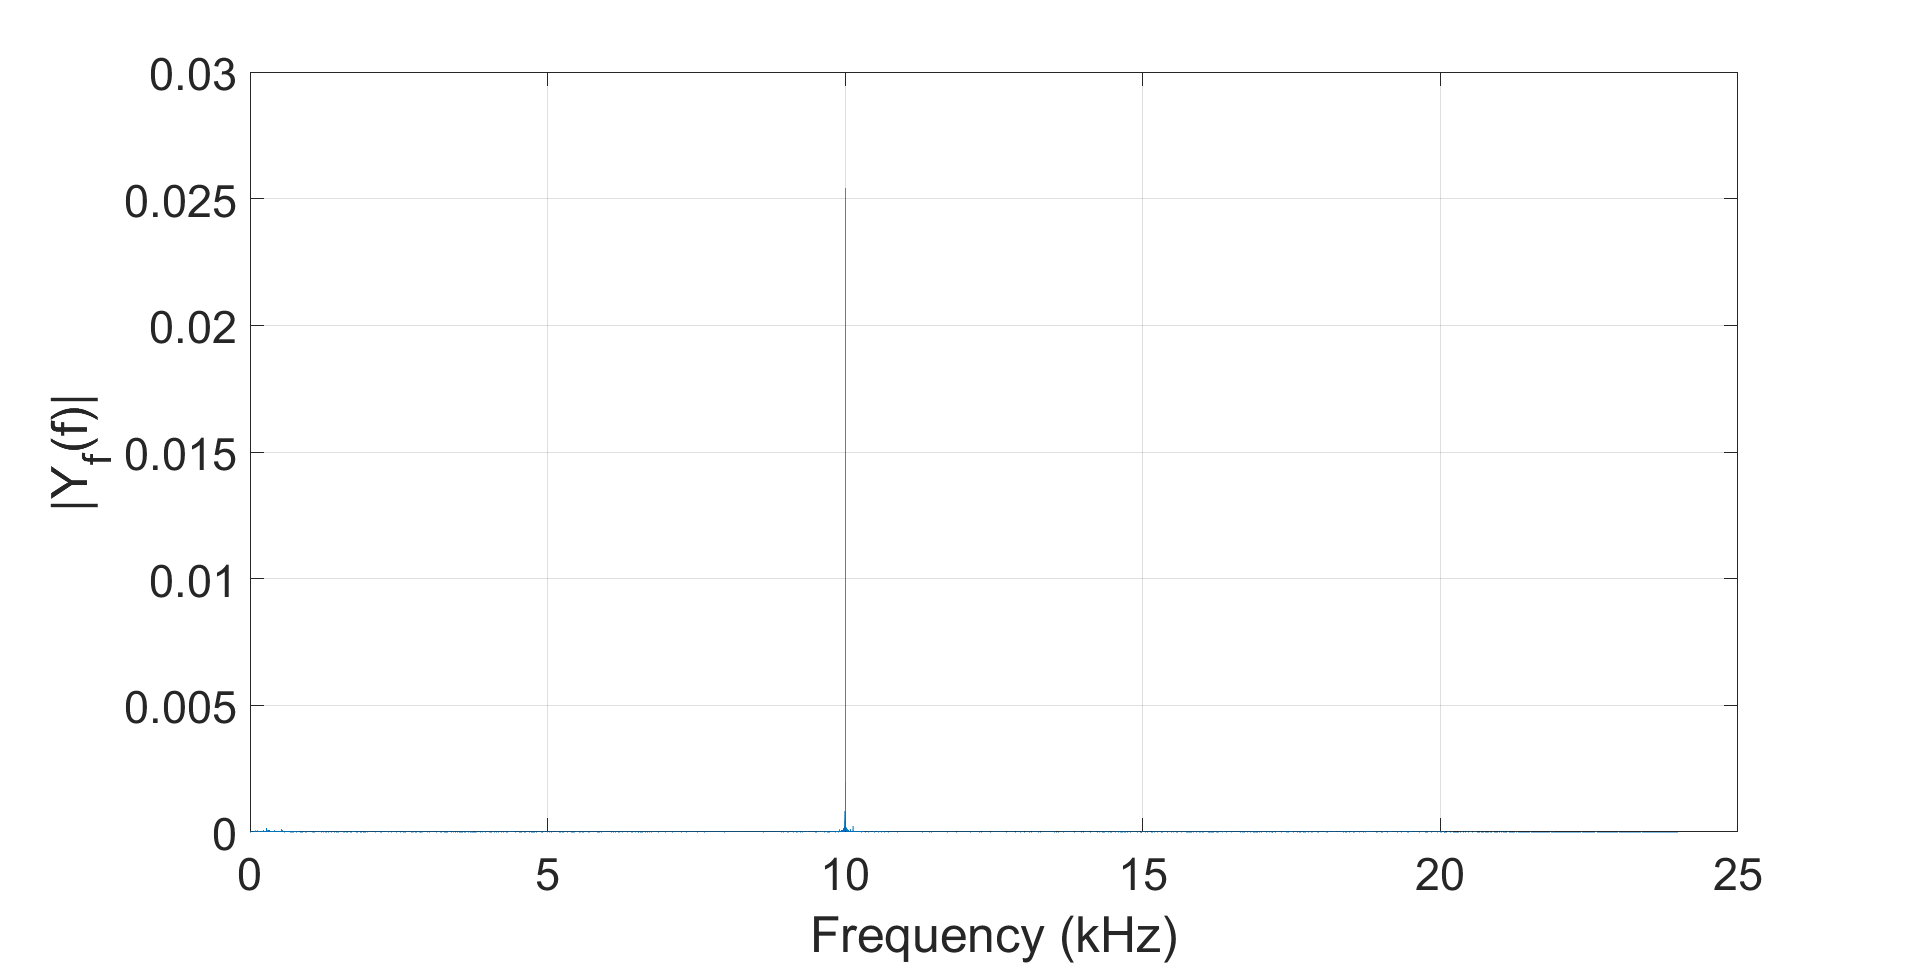
\includegraphics[width=0.5\textwidth]{./images/speaker/L_Output}
	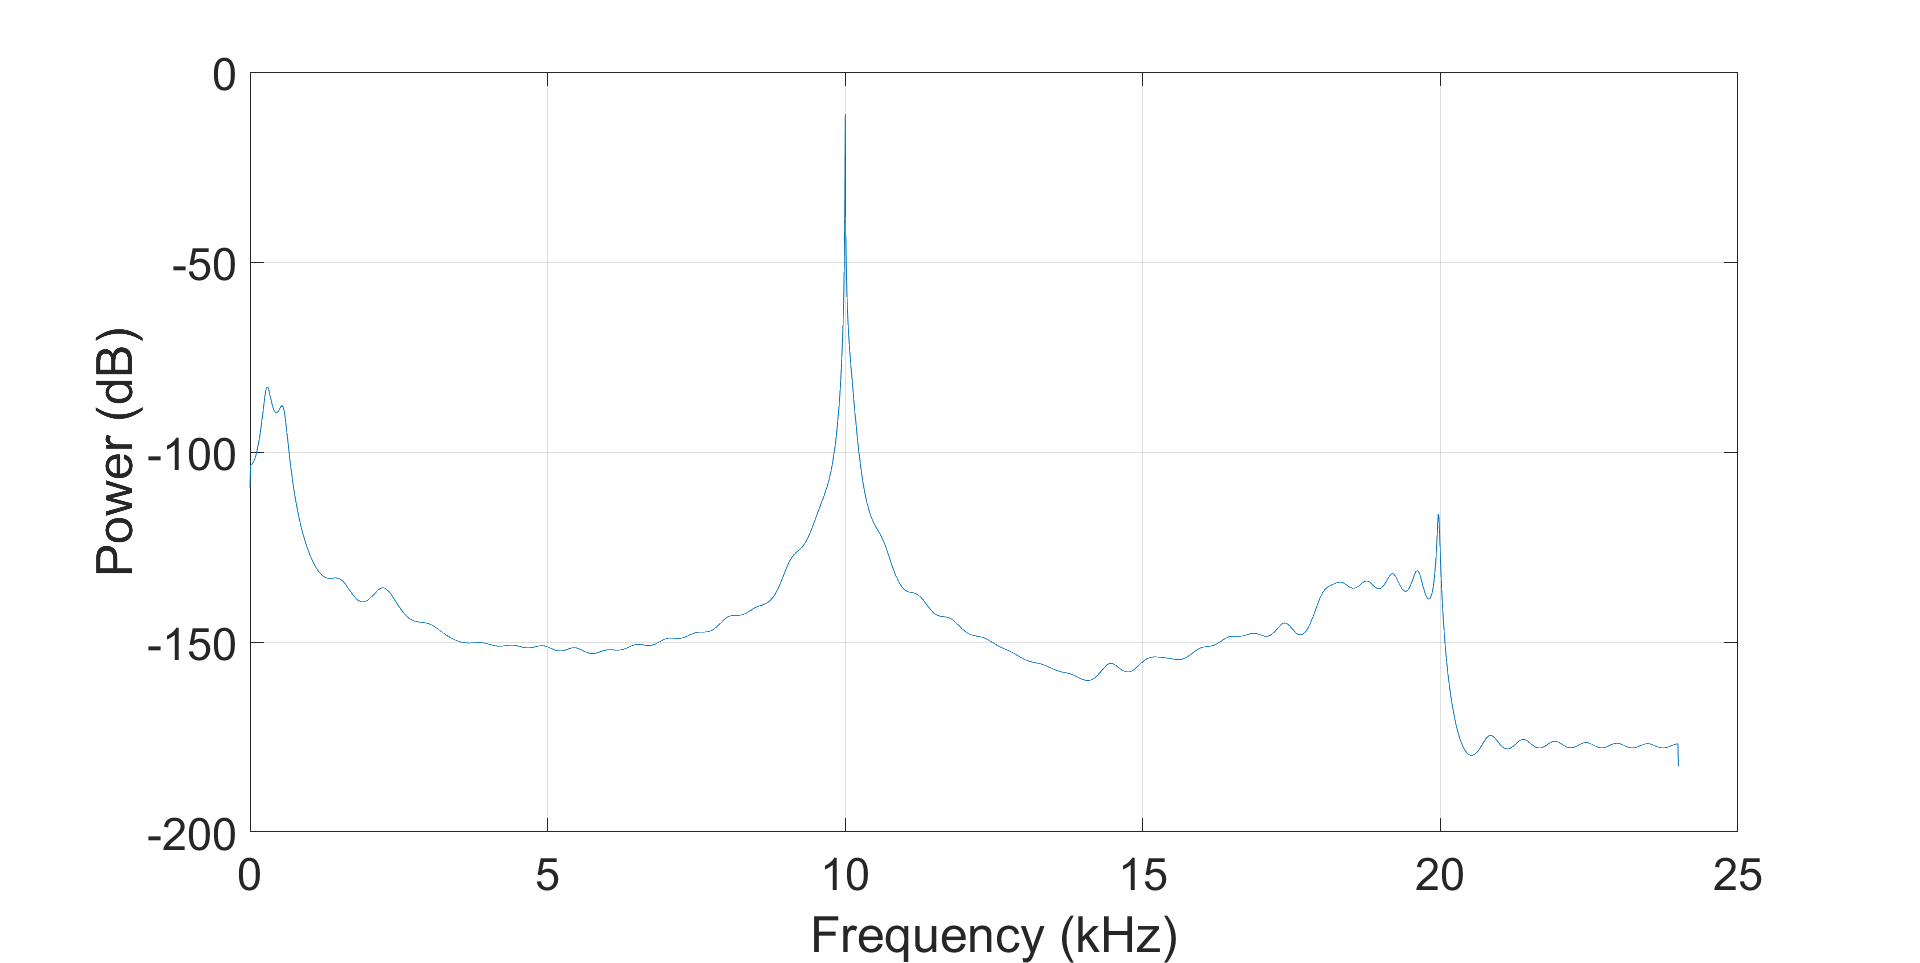
\includegraphics[width=0.5\textwidth]{./images/speaker/L_output_PSD}
	\caption{Left: the output audio spectrum. Right: the output power spectral density (PSD)}
	\label{fig:L_Output}
\end{figure}

\pagebreak
\subsection{Discussion}
The objective for the speaker system was to produce a system that can play a loud and accurate tone. Control for the system should be easily used to produce any desired tone within the speakers range. The system developed should meet as many of the user requirements as possible. \\

The system for generating waveforms works well. By utilising waveforms and using functions from within the serial interface, a wide range of tones were able to be quickly tested. In the testing phase with the other devices, using waveforms allowed ease of talking between devices. Use of waveforms could be useful in final product. A device could play a waveform and if no results are picked up, the device could move on and play another waveform. Devices could also be given unique waveforms, potentially allowing several devices to talk at the same time as each other. \\

The amplifier is a class D amplifier which means that the output is a square waveform. To compensate for this, an additional 2nd order LPF can be added to the legs of the speaker. However, the speaker itself acts as a low pass filter with a cut-off of 20kHz. This means that the only use of the filters will be for reducing electromagnetic interference and as a result were not implemented in the final system for the speaker. To improve on the reliability of the system however, these LPF should be implemented. \\

The final hardware design is big which means it does not meet the small design user requirement. As this system was designed with testing in mind, it serves its purpose. The designed system is ultimately just a prototype and would need to be refined and polished. For future development, it is recommended to construct a PCB. The PCB should also address the use of the variable resistor as the current trim-pot variable resistor requires direct interaction with the hardware. Using a system that can control the output audio using code would be beneficial for further development of the system, allowing for freedom of control of the output audio power. \\

Development of the sinusoidal PWM system took longer than it should have. It would make more sense in the final product to utilise a DAC chip or a MCU with an onboard DAC. This would result in a system that is not so reliant on the fast interrupt period. If a DAC chip had been purchased from the start, the time spent on the sinusoidal PWM could have been spent on other areas such as helping other group members on their development. \\

The system is fully capable of playing tones up to 20kHz, which is the full range of the speaker. This is however with a fast MCU with the 5$\mu$s interrupt (200kHz) used in creating the sinusoidal signal. For a slower MCU clock speeds, this might not be possible. As a result it is even more important for slower micros to use an off-board or on board DAC for generating the sinusoidal tone.\\

Most of the output signal is concentrated within the central 10kHz lobe as shown in Figure \ref{fig:L_Output}. The PSD shows this more clearly, where there is peak at lower frequencies due to background noise at the time of recording. Although, since the unit of the PSD is in dB, the noise is completely dominated by the output signal. The speaker system is therefore capable of playing accurate tones as the design requirements. Further testing would need to be conducted on the speaker system to identify the exact limitations of the system. \\

The prototype system for the speaker is complete and the framework has been laid to allow for ease of integration with the rest of the system. \\